\documentclass[10pt]{ctexbeamer}
\usepackage{bm}
\usepackage{tikz}
\usepackage{amsmath}
\usepackage{graphicx}
\newfontfamily{\dengxian}{DengXian}
\newCJKfontfamily{\fzyaoti}{FZYaoTi} %方正姚体
\newCJKfontfamily{\fzjinghong}{FZZJ-JHTJW} %方正字迹-惊鸿体
\newCJKfontfamily{\dqheiti}{Hiragino Sans GB} %冬青黑体
\newCJKfontfamily{\fandolhei}{FandolHei}

% \usetheme[color blocks]{Verona}% 使用Verona主题
% \usetheme[color blocks, red]{Verona}% 使用Verona主题, red theme
% \usetheme[color blocks, gray]{Verona}% 使用Verona主题, grey theme
\usefonttheme[onlymath]{serif}% 数学公式字体设置
\author{Norsesun}
\date{最后更新:\today}
\logo{
\includegraphics[height=1.2cm]{../../../Pngtree owl double exposure.png}}

\definecolor{airforceblue}{rgb}{.36,.54,.66}



\newcommand{\bmc}[1]{$\bm{#1}$}%定义一个新命令,行内数学模式的粗体,使幻灯片上的公式更清楚
\newcommand{\bmcc}[1]{
        \begin{displaymath}
            \bm{#1}
        \end{displaymath}
    }%定义一个新命令,行间数学模式的粗体,使幻灯片上的公式更清楚
\newcommand{\makecenter}[1]{\vspace{0.5em}\centering \parbox{.6\textwidth}{#1}}%定义一个新命令,居中排布一段话
\newenvironment{Mathbreakcenter}[1][1mm]{
        \par
        \vspace{#1} 
        \centering

    }{
        \par
        \vspace{2mm}
    }
\newcommand{\myblock}[3][1-]{
    \centering
    \begin{minipage}{.6\textwidth}
        \begin{block}<#1>{#2}%
            \centering%
            #3
        \end{block}
    \end{minipage}  
    } %定义一个新命令,居中排布一个block

    \newcommand{\myalertblock}[3][1-]{
        \centering
        \begin{minipage}{.6\textwidth}
            \begin{alertblock}<#1>{#2}%
                \centering%
                #3
            \end{alertblock}
        \end{minipage}  
        } %定义一个新命令,居中排布一个alertblock
\newcommand{\cleave}[2]{
    \hbox to #1{} #2 \hbox to #1{}
}
% \newcommand{\annmark}[1]{%
%     \textcolor{red}{$\bm\langle$#1$\bm\rangle$}%
% }%

% \newcommand{\ann}[1]{%
%     \begin{tikzpicture}[remember picture, baseline=-0.75ex]%
%         \node[coordinate] (inText) {};%
%     \end{tikzpicture}%
%     \marginpar{%
%         \renewcommand{\baselinestretch}{1.0}%
%         \begin{tikzpicture}[remember picture]%
%             \definecolor{orange}{rgb}{1,0.5,0}%
%             \draw node[fill=red!20,rounded corners,text width=\marginparwidth] (inNote){\footnotesize#1};%
%     \end{tikzpicture}%
%     }%
%     \begin{tikzpicture}[remember picture, overlay]%
%         \draw[draw = orange, thick]
%             ([yshift=-0.2cm] inText)
%                 -| ([xshift=-0.2cm] inNote.west)
%                 -| (inNote.west);%
%     \end{tikzpicture}%
% }%

% \setlength{\marginparwidth}{2.5cm}
% \renewcommand{\baselinestretch}{1.3}

\newenvironment{mathsalvation}[2][{解:}]{
    \begin{center}{}
        \begin{minipage}[t]{.05\textwidth}
            \vspace{0pt}
            {\color{#2}{#1}} \quad 
        \end{minipage}
        \begin{minipage}[t]{.7\textwidth}
            \vspace{0pt}
            % \fzyaoti
            % \dengxian
            % \fzjinghong
            % \dqheiti
            \fandolhei
}{
    \end{minipage}
    \end{center}
}

\usepackage{smartdiagram}
\usepackage{multirow}
\usepackage{hyperref}
\usepackage{multicol}

\usetikzlibrary{mindmap}
\title{第一章的复习}
\subtitle{Review of Chapter 1}

\setbeamertemplate{section in toc}[sections numbered]
% \setbeamercolor{normal text}{bg=red!20}
\AtBeginSubsection[\star]
{
	\begin{frame}{要点目录}
		\tableofcontents[currentsubsection]
	\end{frame}
}

\usefonttheme{default}

\begin{document}
    \frame{\titlepage}
    \begin{frame}
        \begin{figure}
            \smartdiagramset{
                distance planet-satellite=3cm,
                satellite text width=2cm
                }
            \smartdiagram[connected constellation diagram]{
            有理数, 1. 有理数的分类, 2. 有理数的相关概念, 
            3. 有理数的大小比较, 4. 有理数的运算
            }
        \end{figure}
    \end{frame}

    \section{有理数}
    \subsection{有理数的定义}
    \boldmath
    \begin{frame}[c]{有理数(Rational Number)}
        \begin{alertblock}{}
            整数与分数统称为\alert{有理数}。
        \end{alertblock}
        
        \begin{columns}
            \column{0.5\textwidth}
           
                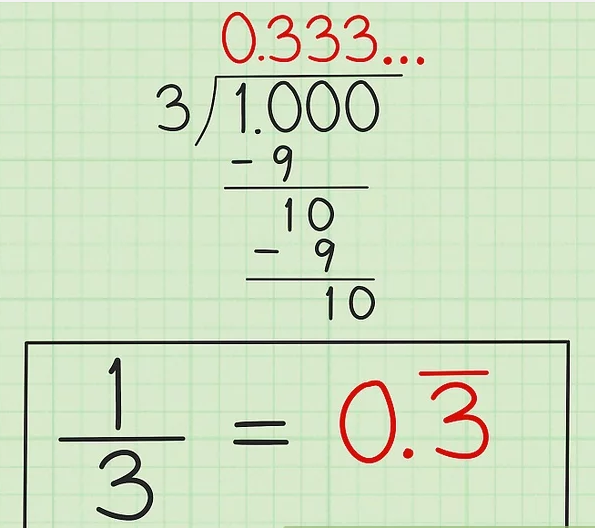
\includegraphics[width=0.37\textwidth]{assets/1 over 3.png}
            
            \only<1>{
                \begin{block}{可以把有理数看做分数吗?}
                    把整数看成是分母为1的分数,
                    那么一个有理数代表着一个形如
                    $\frac{p}{q}$ (其中$p$,$q$为整数)的分数。\alert{
                        有理数都可以表示成两个整数之比}。
                \end{block}
                $\pi$ 无法表示成两整数之比。$\pi$是\alert{无理数}。
                }
            \only<2>{
                \begin{block}{可以把有理数看做无限循环小数吗?}
                    \alert{分数都可以化成无限循环小数或有限小数}。
                    若把有限小数和整数看成是循环节为$0$的无限循环小数,那么
                    一个有理数可以视作一个无限循环小数。
                \end{block}
                $\pi$是无限不循环小数。
            }

            \column{0.48\textwidth}
            \only<1>{
                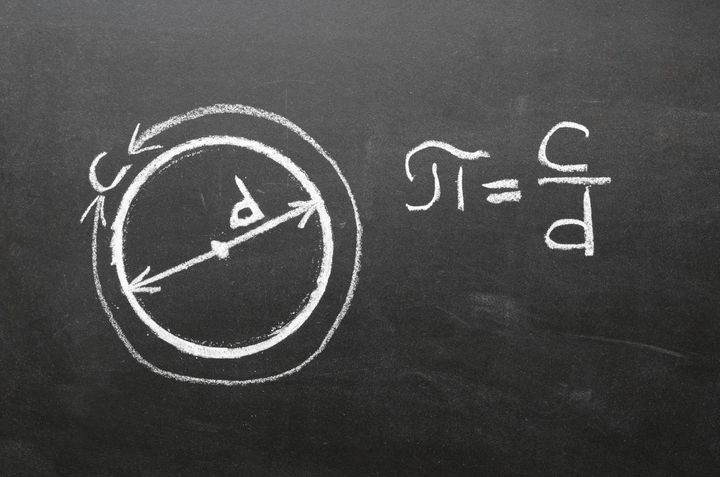
\includegraphics[width=0.99\textwidth]{assets/pi.jpeg}
            }
            \only<2>{ 
                \begin{figure}
                    
                    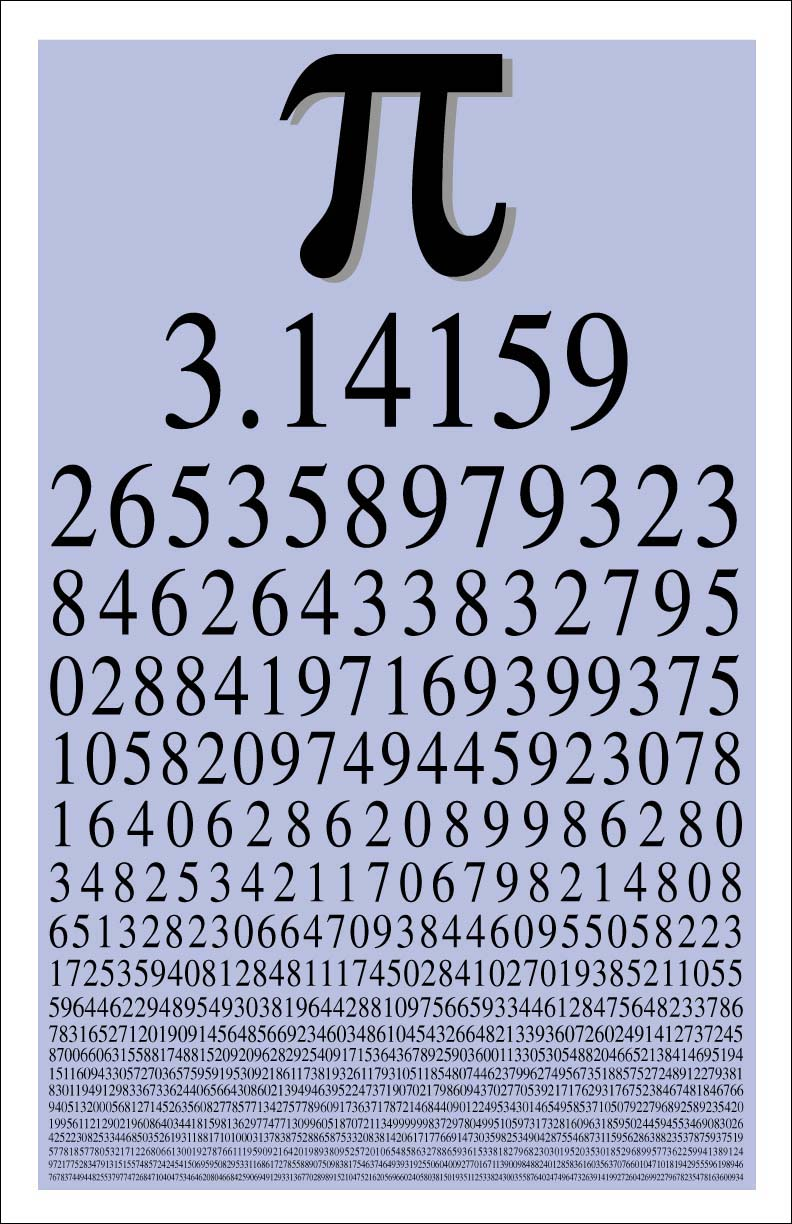
\includegraphics[width=0.59\textwidth]{assets/pi number.jpg}
                \end{figure}
                
            }
        \end{columns}
        
    \end{frame}

    \begin{frame}[shrink=5]{数的发展}{毕达哥拉斯学派相信,一切都可以用整数或整数之比来表示。}
        大约在公元前5世纪,毕达哥拉斯学派的希帕索斯发现了:
        $\sqrt{2}$。
        希帕索斯正是因为这一数学发现,而被毕达哥拉斯学派的人投进了大海,
        处以“淹死”的惩罚。
        \begin{columns}
            \column{0.59\textwidth}
            \smartdiagram[priority descriptive diagram]
                {
                    整数, 分数, 无理数
                }

            \column{0.39\textwidth}
            \begin{quotation}[毕达哥拉斯 Pythagoras]
                万物皆数(All is Number)。
            \end{quotation}
            \begin{figure}
                \centering
                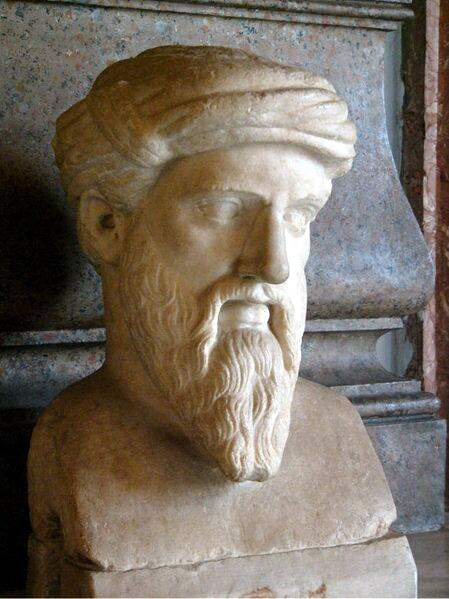
\includegraphics[width=0.6\textwidth]{assets/Kapitolinischer_Pythagoras_adjusted.jpg}
            \end{figure}
        \end{columns}
        
    \end{frame}

    \begin{frame}{例题1}{知识点:整数,分数,有理数}
        \begin{block}{}
            $0.9999999999$, $-\dfrac{1}{3}$, $0$, $\pi$中有几个
            有理数?有几个整数?\\ 请你从语文的角度理解“整” 与 “分” 的含义。
        \end{block}

        \pause $0.9999999999$, $-\dfrac{1}{3}$, $0$ 是有理数。\\
        其中 $0$ 是整数。
    \end{frame}

    \subsection{有理数的分类}
    \begin{frame}{有理数的分类}
            {$\pi$ 不是有理数; $0$既不是正数也不是负数; $-3.1415926$属于什么数?}
        \begin{figure}
            \begin{tikzpicture}
                % [mindmap, 
                % concept color=green!30,scale=0.8,
                % level 1 concept/.append style =
                %     {font=\Large\bfseries, sibling angle=90},
                % level 2 concept/.append style =
                %     {font=\normalsize\bfseries},
                % level 3 concept/.append style =
                %     {font=\small\bfseries},
                % ]
            [
                every node/.style={
                    draw=blue!70,rounded corners
                },
                grow cyclic,
                edge from parent/.style={blue, thick, draw},
                level 1/.style={level distance=2.5cm,
                    sibling angle=90, fill=green!20},
                level 2/.style={level distance=2cm,sibling angle=45}
            ]
            
            \node {有理数}
                child [grow=45, color=red!60]
                {
                    node {正有理数} 
                    child{node{正整数}}
                    child{node{负整数}}
                }
                child[grow=right, color=red!60]{node{零}}
                child[grow=-45, color=red!60]{
                    node{负有理数}
                    child[grow=right]{node{负整数}}
                    child[grow=30]{node{负分数}}
                }
                child[grow=135]{
                    node{整数}
                    child{node{正整数}}
                    child{node{零}}
                    child{node{负整数}}
                }
                child[grow=225]{node{分数}
                    child[grow=left]{node{正分数}}
                    child[grow=150]{node{负分数}}
                };
            \end{tikzpicture}
        
    \end{figure}
    \end{frame}

    \begin{frame}{例题2}{知识点:有理数的分类}
        \begin{block}{}
            把 $ -\dfrac{1}{2}$, $+5$, $-6.3$, $0$, 
        $-\dfrac{12}{13}$,$6.9$,
        $-7$, $210$, $0.031$,$-43$, $-10\%$ 填入对应的集合。
        \end{block}
        
        \begin{columns}
            \column{.59\textwidth}
            正数集合: \underline{\makebox[10em]{
                \only<2->{
                    $+5$, $0.9$, $210$, $0.031$
                }}} \\
            整数集合:\underline{\makebox[10em]{
                \only<2->{$+5$, $0$,$-7$, $210$, $-43$}
                }} \\
            非负数集合:\underline{\makebox[10em]{
                \only<2->{ $+5$, $0.9$, $210$, $0.031$, $0$}
            }} \\
            负分数集合:\underline{\makebox[10em]{
                \only<2->{$ -\dfrac{1}{2}$, $-6.3$, $-\dfrac{12}{13}$,
                $-10\%$
                }
            }} \\

            \column{.29\textwidth}
            \framebox{正数和零统称\alert{非负数}。}
        \end{columns}
        
    \end{frame}

    \subsection{有理数的相关概念}
    \begin{frame}{有理数的相关概念}{数轴、相反数和绝对值的定义以及它们的数学写/画法}
        \begin{figure}
            \centering
            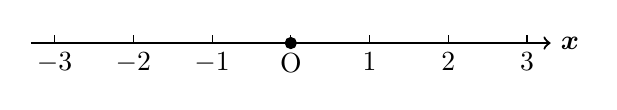
\begin{tikzpicture}
            
                \draw [->, thick] (-3.3, 0) 
                    --(0, 0) node[below]{O}
                    -- (3.3,0) node[right]{\bmc{x}};
                \draw [fill=black](0, 0) circle (2pt);
    
                \foreach \x in {-3, -2, -1, 1, 2, 3}
                    \node [below] (w1_\x) at (\x, 0)
                        {$\x$};
                \foreach \x in {-3, ..., 3}
                    \draw (\x, 0) -- (\x, 0.1);
            \end{tikzpicture}
        \end{figure}
        
        \begin{columns}
            \column{0.45\textwidth}
            \begin{tikzpicture}
                [mindmap, grow cyclic, every node/.style=concept, 
                    concept color=orange!40, 
                    level 1/.style={level distance=3cm,sibling angle=40},
                ]
                \tikzstyle{every node}=[font=\normalsize, scale=0.6, concept]
                \node{有理数相关概念}
                child [concept color=blue!30]{ 
                    node {绝对值\\(Absolute Value)\\ \bmc{x}的绝对值写作\bmc{|x|}。}
                }
                child [concept color=red!30]{ 
                    node {相反数\\(Opposite Number)\\\bmc{x}的相反数写作\bmc{-x}。\\
                    \bmc{-x}表示负数还是正数?}
                }
                child [concept color=green!30]{ 
                    node {数轴(Number Axis)\\三要素:原点(Origin),正方向,单位长度。} 
                };
            \end{tikzpicture}

            \column{0.53\textwidth}
            \only<1>{
                \textbf{数轴}:原点代表$0$,一般以向右为正方向,单位长度要统一。
                \begin{block}{数轴表示数}
                    \alert{任何}有理数都可以用数轴上\alert{唯一}的一个点表示。
                \end{block}
                \begin{block}{相反数}
                    \alert{只有}符号不同的两个数,互为相反数。
                \end{block}
            }
            \only<1>{比如 $-1$ 和 $1$。互为相反数的两个\\数在数轴上怎么排布?}
            \only<2, 4>{
                \begin{alertblock}{数轴与相反数}
                    互为相反数的两个数在数轴上\alert{关于原点对称}。$0$ 的相反数是 $0$。
                \end{alertblock}
            }
            \only<2, 3>{
                \begin{block}{绝对值}
                一个数的绝对值无关于这个数的符号,是这个数对应的\alert{非负的值}。
                \end{block}
            }
            \only<3>{
                \begin{quotation}
                    正数的绝对值是它本身;\\
                    负数的绝对值是它的相反数;\\
                    0的绝对值是0。
                \end{quotation}

                有没有更好地方式去理解绝对值?
            }
            \only<4>{
                \begin{alertblock}{数轴与绝对值}
                    一个数的绝对值等于数轴上表示这个数的点\alert{到原点的距离}。
                    0的绝对值是0。
                \end{alertblock}

                \small{用数学表达式表示一个数的绝对值\\(比如\bmc{|a|})去掉绝对值符号后的结果?}
            }
        \end{columns}
    \end{frame}

    \begin{frame}{例题3}{知识点:相反数与绝对值}
        \begin{columns}
            \column{0.29\textwidth}
            \begin{figure}
                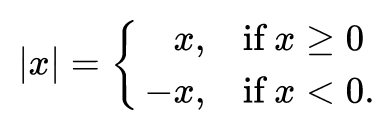
\includegraphics[width=0.99\textwidth]{assets/abs func.png}
            \end{figure}

            \column{0.69\textwidth}
            \begin{block}{}
                $ -(-5 ) $ 等于多少?它的相反数又是多少?它和它的相反数的绝对值分别是多少?有什么规律?
            \end{block}

            \only<2>{
                \textbf{答:}
                \begin{columns}
                    \column{0.39\textwidth}
                    $ -(-5 ) = 5 $ 
                    \column{0.59\textwidth}
                    \framebox{\small{去括号的规则适用于这里吗?}}
                \end{columns}
               
                它的相反数为 $ -(-(-5)) = -5 $,\\
                它和它的相反数的绝对值如下:\\
                    \begin{columns}
                        \column{0.29\textwidth}
                        $|5| = 5$ \\
                        $|-5| = 5$
                        \column{0.69\textwidth}
                        \framebox{\small{去括号与去绝对值符号有什么不同?}}
                    \end{columns}
                    
            }
        \end{columns}
        \unboldmath
        \only<2>{
            \begin{alertblock}{}
                我们发现,互为相反数的两个数,绝对值相等。即 
                \alert{\bmc{|-a| = |a|}}。
            \end{alertblock}
        }
    \end{frame}

    \begin{frame}[shrink=5]{例题4}{知识点:绝对值的非负性,绝对值的几何含义拓展}
        
        \only<1, 2, 3>{
            % \begin{alertblock}{}
            %     互为相反数的两个数,绝对值相等。即 
            %     \alert{\bmc{|-a| = |a|}},\alert{\bmc{|a-b| = |b-a|}}。
            % \end{alertblock}
            \begin{figure}
                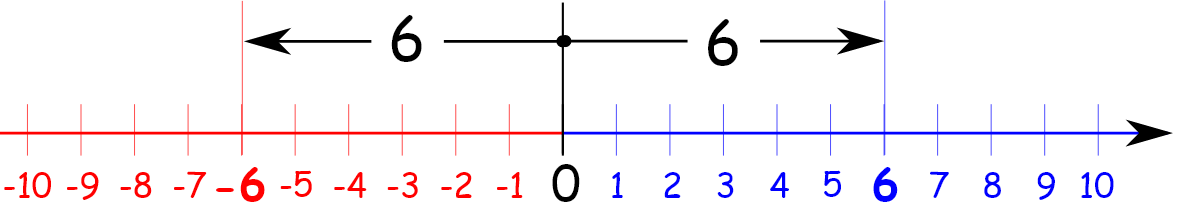
\includegraphics[totalheight=1.5cm]{assets/abs.png}
            \end{figure}
            
        }
        \begin{columns}[t]
            \column{0.48\textwidth}
            \begin{block}{}
                已知 \bmc{|x-1| + |y+4|=0},求\bmc{xy}。
            \end{block}

            \only<2->{
                \textbf{解:} 因为 \bmc{|x-1|\geq 0} 且
                    \bmc{|y+4|\geq 0} \\
                    \qquad 故 
                    \[
                    \begin{cases}
                        x-1=0 , x=1\\
                        y+4=0 , y=-4
                        \end{cases}
                    \]
                    \qquad 所以 \bmc{xy=(1)\times(-4)=-4}
            }

            \column{0.48\textwidth}
            \begin{block}{}
                \bmc{a-b}与 \bmc{b-a}有什么数量关系?
                二者的绝对值具有什么几何意义?
            \end{block}
            
            \only<2->{
                \textbf{解:} 
                    因为\\ \small{\bmc{-(a-b)=-a+b=b+(-a)=b-a} ,即
                    \alert{\bmc{-(a-b)=b-a}}。
                    所以\bmc{a-b}与\bmc{b-a}
                    互为相反数。} \\ 
            }
            \only<3>{
                \bmc{|a-b|=|b-a|},\small{在数轴上表示\\
                    \alert{$a$,$b$两点的距离}。举例验证。}
            }
        \end{columns}
    \end{frame}

    \begin{frame}{例题5}{知识点:绝对值}
        \begin{columns}
            \column{0.48\textwidth}
                \begin{block}{}
                    已知 \bmc{|a| + |b|=9},且 \bmc{|a|=2}, 
                求 $b$ 的值。
                \end{block}

            \column{0.48\textwidth}
            \begin{block}{}
                已知\bmc{|a|=3}, \bmc{|b|=2}, 
                \bmc{|c|=1}, 且\bmc{a<b<c}, 求\bmc{a},$b$,$c$的值。
            \end{block}
        \end{columns}
    \end{frame}

    \subsection{有理数大小的比较}
    \begin{frame}{有理数大小的比较}{负数大小比较:先求绝对值,再比较大小}
        \only<1>{
            \begin{tabular}{|c|p{2.5cm}|p{5cm}|}
                \hline
                知识点 & 摘要 & 示例 \\
                \hline
                \multirow{3}*{利用法则\newline 比较两数大小} & 正数大于0,0大于负数,正数大于负数 & 如$7$与$-7$,$7>0,0>-7$,故$7>-7$。\\
                \cline{2-3}
                & 两个正数比较,绝对值大的数较大。&如$9.6$与 $6.9$,由于$|9.6|>|6.9|$,所以$9.6>6.9$。\\
                \cline{2-3}
                & \alert{两个负数比较,绝对值大的反而小} & 如$-5$和$-3$,由于$|-5|>|-3|$,所以$-5<-3$。\\
                \hline
            \end{tabular}
        }
        \only<1->{
            \begin{figure}
                \centering
                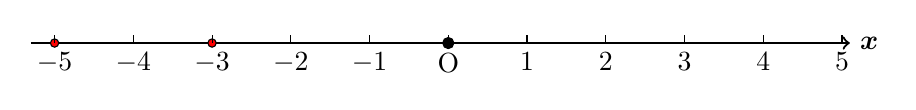
\begin{tikzpicture}
                
                    \draw [->, thick] (-5.3, 0) 
                        --(0, 0) node[below]{O}
                        -- (5.1,0) node[right]{\bmc{x}};
                    \draw [fill=black](0, 0) circle (2pt);
                    \draw [fill=red](-5, 0) circle (1.5pt);
                    \draw [fill=red](-3, 0) circle (1.5pt);
        
                    \foreach \x in {-5, -4, -3, -2,-1, 1, 2, 3, 4, 5}
                        \node [below] (w1_\x) at (\x, 0)
                            {$\x$};
                    \foreach \x in {-5, ..., 5}
                        \draw (\x, 0) -- (\x, 0.1);
                \end{tikzpicture}
            \end{figure}
        }
        \only<2->{
            \begin{alertblock}{}
                在以向右为正方向的数轴上,右边的点表示的数比左边的点表示的数大。
            \end{alertblock}
            \begin{figure}
                \only<2>{
                    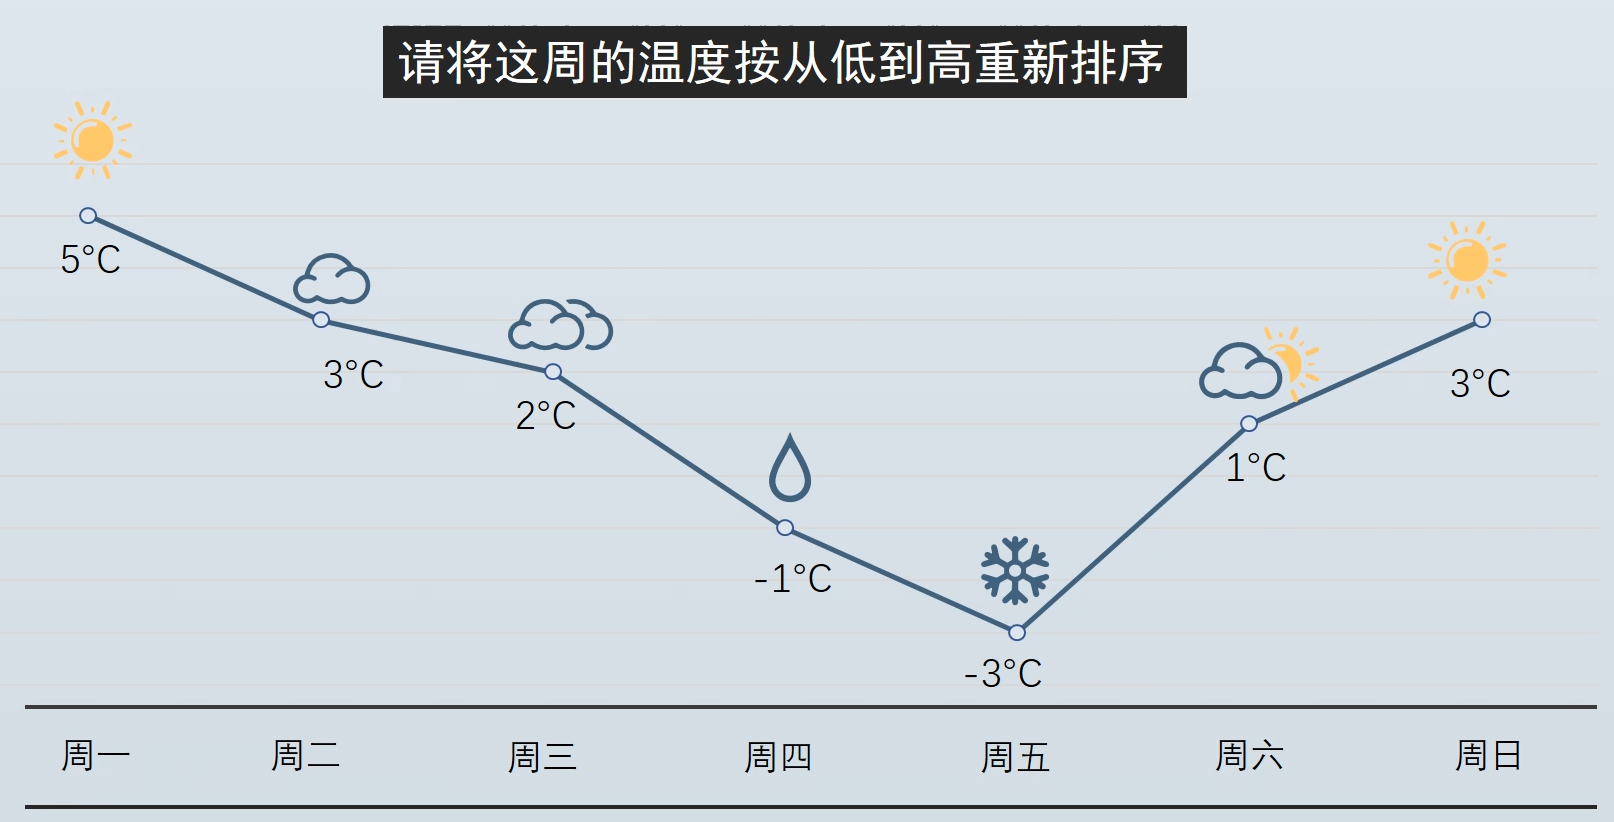
\includegraphics[width=.67\textwidth]{assets/temp.png} 
                }
                \only<3>{
                    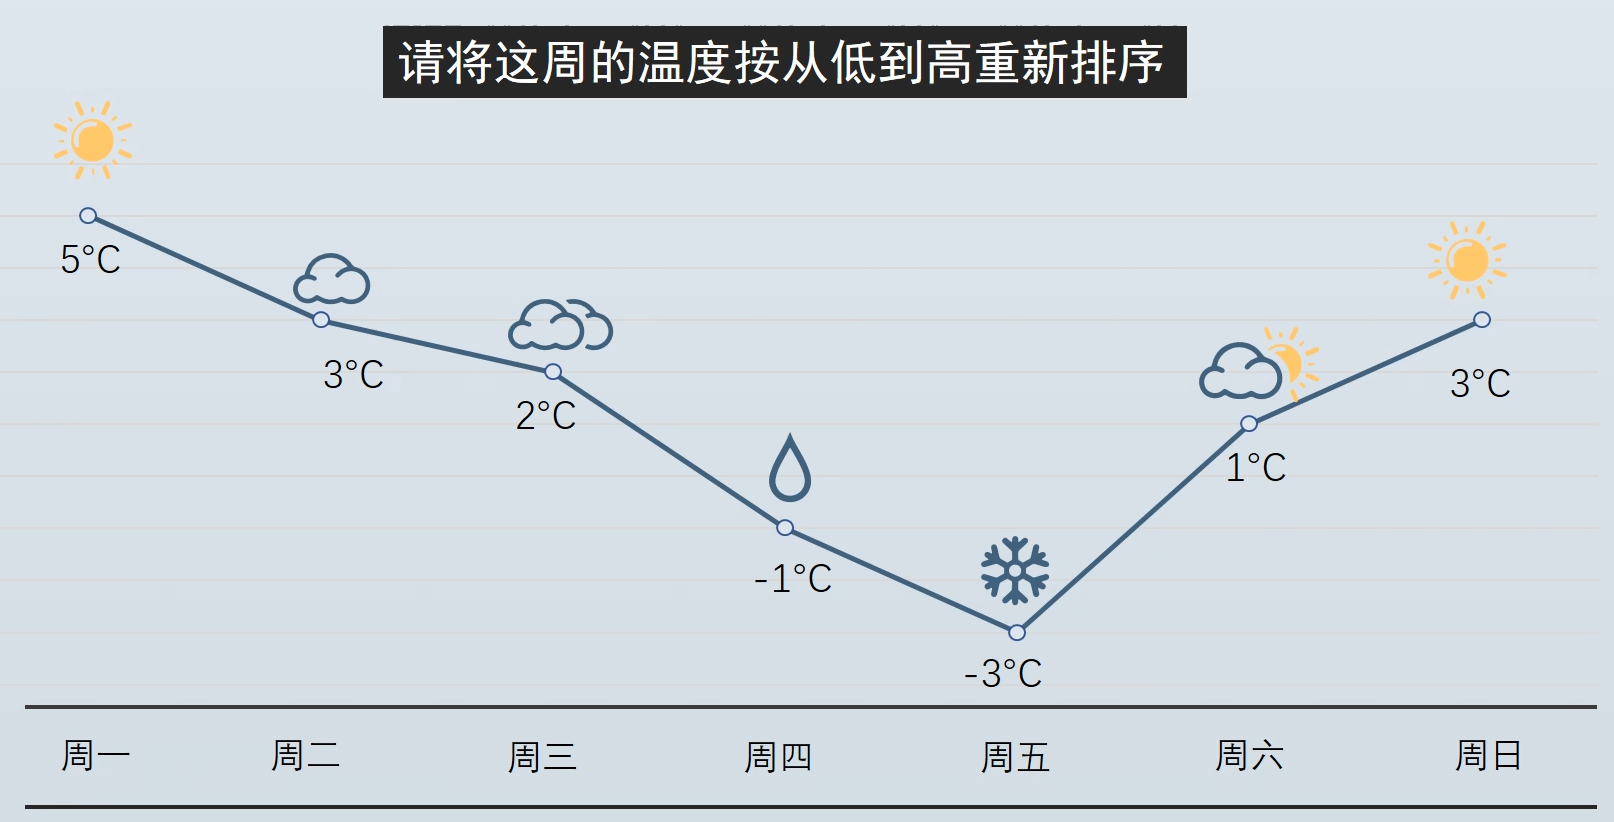
\includegraphics[width=.49\textwidth]{assets/temp.png} 
                    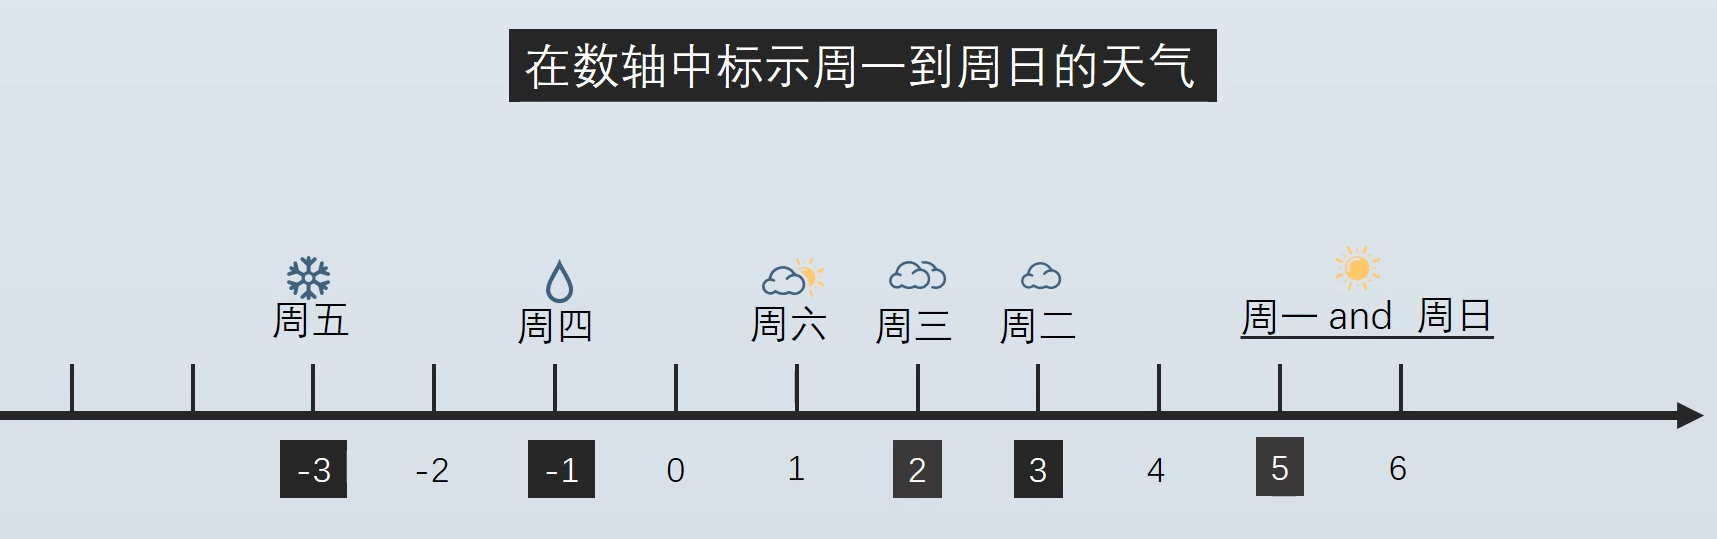
\includegraphics[width=.49\textwidth]{assets/temp2.png}}
                \caption[*]{生活中的例子:温度}
            \end{figure}
        }
    \end{frame}
    \begin{frame}{例题6}{知识点:相反数,绝对值与大小比较}
        \begin{columns}
            \column{0.48\textwidth}
            \begin{block}{比较下列两组数的大小:}
                \bmc{-\dfrac{2}{3}} 与 \bmc{-\dfrac{3}{4}}\\
                \bmc{|-(+2.1)|} 与 \bmc{-(-2.1)}
            \end{block}
            \begin{block}{看右图:}
                已知有理数\bmc{a} 与 \bmc{b}
                在数轴上如右图所示,请比较\bmc{a}, \bmc{b},
                \bmc{-a},\bmc{-b}的大小。
            \end{block}
            \column{0.48\textwidth}
            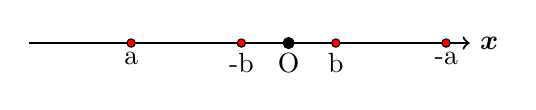
\begin{tikzpicture}
                \draw [->, thick] (-3.3, 0) 
                    --(0, 0) node[below]{O}
                    -- (2.3,0) node[right]{\bmc{x}};
                \draw [fill=black](0, 0) circle (2pt);
                \draw [fill=red](-2, 0) circle (1.5pt) node[below]{a};
                \draw [fill=red](0.6,0) circle (1.5pt) node[below]{b};
                \only<2>{
                    \draw [fill=red](2, 0) circle (1.5pt) node[below]{-a};
                    \draw [fill=red](-0.6, 0) circle (1.5pt) node[below]{-b};
                }
            \end{tikzpicture}
                用小于号连接如下:\\
                \only<2>{
                    \centering
                    \bmc{a<-b<b<-a}
                }
        \end{columns}
    \end{frame}
    \begin{frame}[plain, noframenumbering, label=Question]
        
        \begin{center}
            \Huge{你get到了吗?}
        \end{center}
        \begin{figure}
            
\includegraphics[width=0.2\textwidth]{../../../general assets/wha.jpg}
        \end{figure}
    \end{frame}
    
    \begin{frame}[fragile]
        \begin{columns}
        \column{0.35\textwidth}
        \begin{center}
            \Large{你get到了吗?}
        \end{center}
        \begin{figure}
            
\includegraphics[width=0.4\textwidth]{../../../general assets/wha.jpg}
        \end{figure}
            
            \column{0.63\textwidth}
                \smartdiagram[descriptive diagram]{
                    {有理数的定义, 可以表示成两个整数之比的数。},
                    {有理数的分类, {按符号分为正有理数,零,负有理数,还可以分为整数和分数。}},
                    {相反数绝对值, 结合数轴加深对概念的理解。},
                    {比较大小, {两个负数,绝对值大的反而小}},
                }
        \end{columns}
        \begin{center}
            \small{我们都没有勤奋到要拼天赋的时候。}
        \end{center}
    \end{frame}
% \againframe{Question}
\setbeamercolor{background canvas}{bg=airforceblue}
\begin{frame}[plain]
    \setbeamercolor{postit}{fg=black,bg=airforceblue}
    \begin{beamercolorbox}[ht=2.5cm, sep=1em,wd=\textwidth ,]{postit}
        \centering
        \Huge{回顾!}
    \end{beamercolorbox}
    \begin{figure}
        
\includegraphics[width=0.5\textwidth]{assets/review.png}
    \end{figure}
\end{frame}
\setbeamercolor{background canvas}{bg=white}

\section{有理数的运算}
\subsection{有理数的加减}
\begin{frame}[t]
    \frametitle{加法(Addition)}
    \framesubtitle{异号相加,如果两数的绝对值相等,得$0$。即互为相反数得两数相加为$0$。}
    \begin{theorem}
        \alert<1>{同号相加},符号不变,并把绝对值相加。\\
        \alert<2>{异号相加},取绝对值较大的数的符号,并用大的绝对值减去较小的绝对值。\\
        一个数\alert<1>{同$0$相加},仍得这个数。
    \end{theorem}
    \begin{block}{比如}
        \begin{enumerate}
            \item \bmc{5 + 7 = 12, -5+(-7)=-(5+7)=-12}
            \item<2-| alert@2> \bmc{-5 + 7 = +(7-5)=2, -7 + 5=-(7-5)=-2}
            \item \bmc{0+(-5)=-5}
        \end{enumerate}
    \end{block}
\end{frame}

\begin{frame}[t]
    \frametitle{减法(Subtraction)}
    \framesubtitle{\alert{把减法看成加法},反过来也能把加法看成减法}
    \begin{columns}
        \column{0.48\textwidth}
        \begin{theorem}
            \alert{减去一个数,等于加上这个数的相反数}。\\
            $a\alert{-}b=a\alert{+}(-b)$。
        \end{theorem}

        \column{0.48\textwidth}
        \begin{figure}
            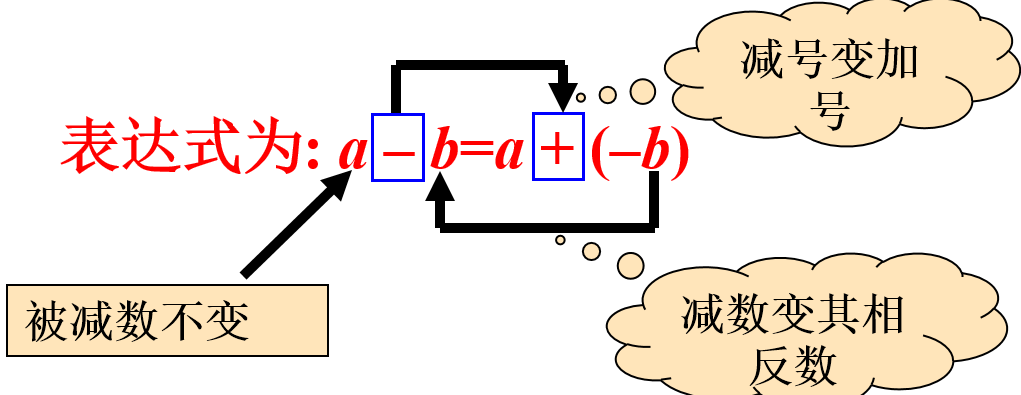
\includegraphics[width=.9\textwidth]{assets/subtraction.png}
        \end{figure}
    \end{columns}

    \only<1>{
    \begin{figure}
        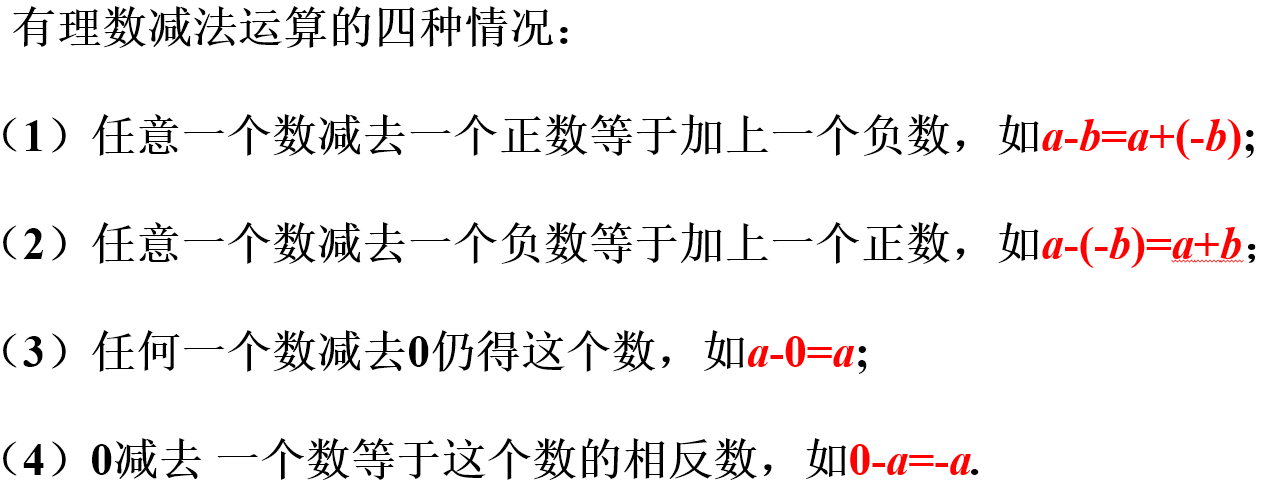
\includegraphics[width=.79\textwidth]{assets/subtraction2.png}
    \end{figure}}
    
    \begin{block}<2>{例题7}
        \begin{enumerate}
            \item \bmc{9 - 8 = }
            \item \bmc{9+(-8)=}
            \item \bmc{15 - 7 = }
            \item \bmc{15 + (-7)=}
        \end{enumerate}
    \end{block}
\end{frame}

\begin{frame}
    \frametitle{加法运算律}
    \framesubtitle{加法交换律(Commutative Law),加法结合律(Associative Law)}
    \begin{columns}
        \column{0.48\textwidth}
        \begin{theorem}
            交换律:\bmc{a + b=b +a}\\
            结合律:\bmc{a + b + c = (a+b)+c=a + (b +c)}
        \end{theorem}
        
        \column{0.45\textwidth}
        减法有交换律吗?像\bmc{a-b= b-a}这样?
    \end{columns}
    \begin{alertblock}<2>{}
        \centering
        \bmc{a -b = -(b-a)}
    \end{alertblock}
    
\end{frame}

\begin{frame}
    \frametitle{例题8}
    \framesubtitle{知识点:减法}
    \begin{block}{}
        今年2月份某市一天的最高气温为 $7^{\circ}$C 度,最低气温为$-3^{\circ}$C 度,那么
        这一天的最高气温比最低气温高多少度?
    \end{block}
\end{frame}

\begin{frame}
    \frametitle{例题9}
    \framesubtitle{知识点:加减法}
    \begin{block}{}
        计算: \bmc{(-2)+(+30)-(-15)-(+27)}
    \end{block}

    \only<2>{
        \begin{figure}
            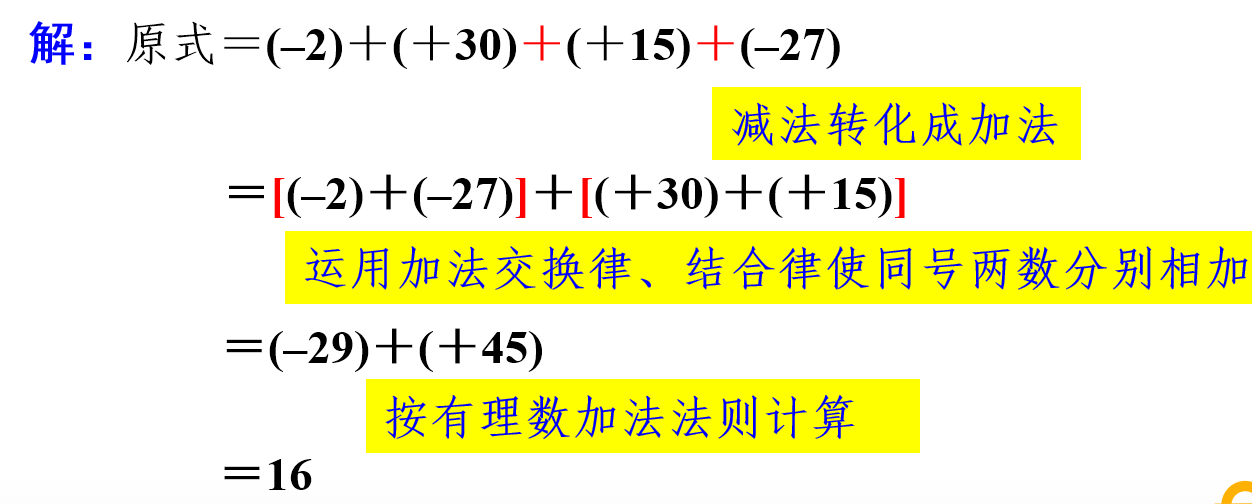
\includegraphics[width=.9\textwidth]{assets/add example1.png}
        \end{figure}
    }
\end{frame}

\subsection{有理数的乘除}
\begin{frame}
    \frametitle{乘法(Multiplication)}
    \begin{columns}
        \column{.59\textwidth}
        \begin{figure}
            
\includegraphics[width=.9\textwidth]{assets/multiplication.png}
        \end{figure}
        \column{.38\textwidth}
        \begin{block}{计算}
            \bmc{2\times3\times4\times(-5)}
            \bmc{2\times3\times(-4)\times(-5)}
            \bmc{2\times(-3)\times(-4)\times(-5)}
            \bmc{(-2)\times(-3)\times(-4)\times(-5)}
            \bmc{2\times3\times4\times(-5)\times0}
        \end{block}
    \end{columns}
    \begin{figure}
        
\includegraphics[width=.69\textwidth]{assets/multiplication2.png}
    \end{figure}
    
\end{frame}

\begin{frame}{乘法运算律}
    \framesubtitle{交换律(Commutative Law),结合律(Associative Law),分配律(Distributive Law)}
    \begin{columns}
        \column{.39\textwidth}
        \begin{block}{}
            \begin{enumerate}
                \item \bmc{ab = ba}
                \item \bmc{(ab)c = a(bc)}
                \item \bmc{a(b+c)= ab+ac}
            \end{enumerate}
        \end{block}

        \column{.59\textwidth}
        \begin{figure}
            \includegraphics<1>[width=.9\textwidth]{assets/law1.png}
            \includegraphics<2>[width=.9\textwidth]{assets/law2.png}
            \includegraphics<3>[width=.9\textwidth]{assets/law3.png}

        \end{figure}
    \end{columns}
    
\end{frame}
\begin{frame}{例题10}{知识点:乘法与乘法运算律}
    \begin{block}{}
        \begin{enumerate}
            \item \bmc{(-\dfrac{3}{4})\times(8-\dfrac{1}{3}-4)}
            \item \bmc{-11\times(-\dfrac{2}{5})+(-11)\times2\dfrac{3}{5}+(-11)\times(-\dfrac{1}{5})}
        \end{enumerate}
    \end{block}

    \begin{figure}
        \includegraphics<2>[width=.79\textwidth]{assets/examp10.png}
    \end{figure}
\end{frame}

\begin{frame}{例题11}{知识点:乘法与乘法运算律}
    \begin{block}{}
        \bmc{(71\dfrac{2}{27})\times(-9)}
    \end{block}

    \begin{figure}
        \begin{flushleft}
            \includegraphics<2>[width=.49\textwidth]{assets/examp11.png}
        \end{flushleft}
        
    \end{figure}
\end{frame}

\begin{frame}{例题12}{知识点:多个数的乘法}

    \begin{figure}
        \begin{flushleft}
            \includegraphics<1>[width=.9\textwidth]{assets/examp12.png}
            \includegraphics<2>[width=.9\textwidth]{assets/examp12-2.png}
        \end{flushleft}
        
    \end{figure}
\end{frame}

\begin{frame}
    \frametitle{倒数(Reciprocal)}
    \framesubtitle{乘积是$1$的两个数互为\alert{倒数}。}
    \begin{figure}
        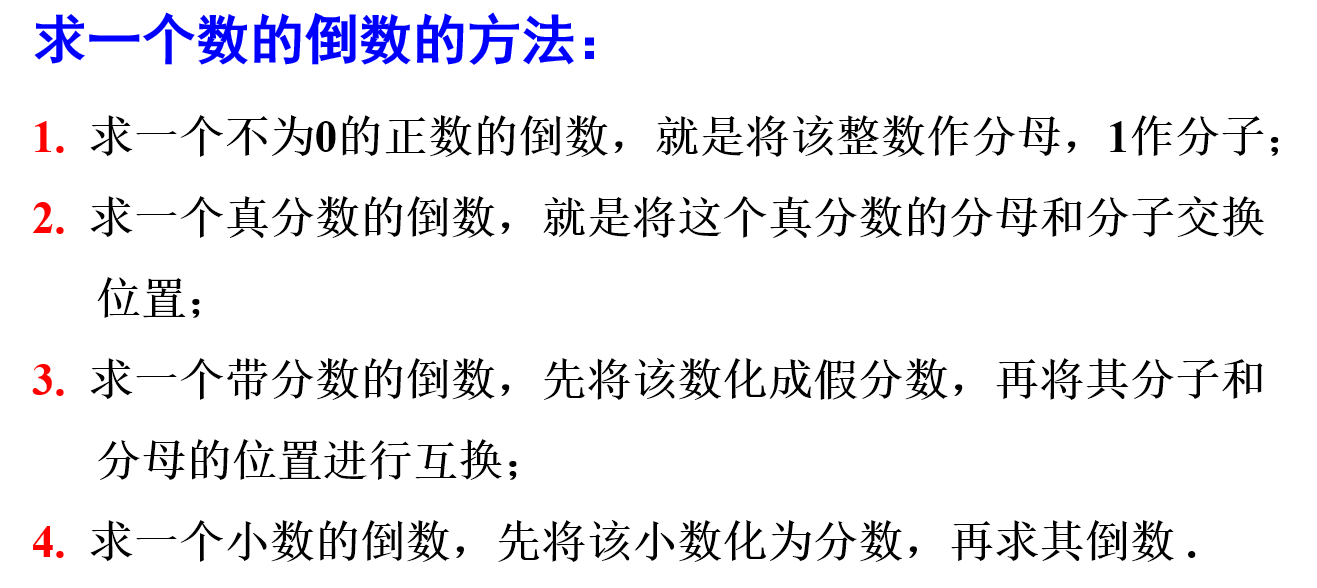
\includegraphics[width=.9\textwidth]{assets/reciprocal.png}
    \end{figure}
    \alert{\bmc{0}没有倒数。因为0乘以任何数都是0,而不可能是1。}
\end{frame}
\begin{frame}
    \frametitle{除法(Division)}
    \begin{columns}
        \column{.49\textwidth}
        \begin{figure}
            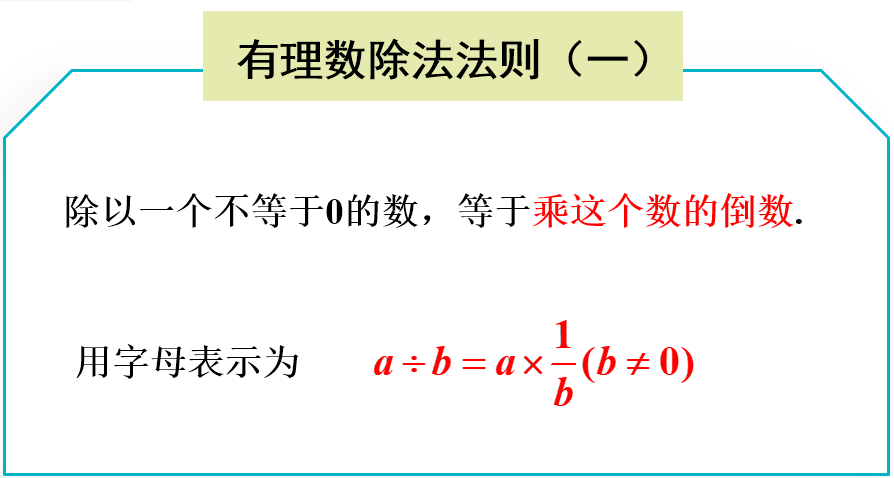
\includegraphics[width=.99\textwidth]{assets/division1.png}
        \end{figure}
        \column{.49\textwidth}
        \begin{figure}
            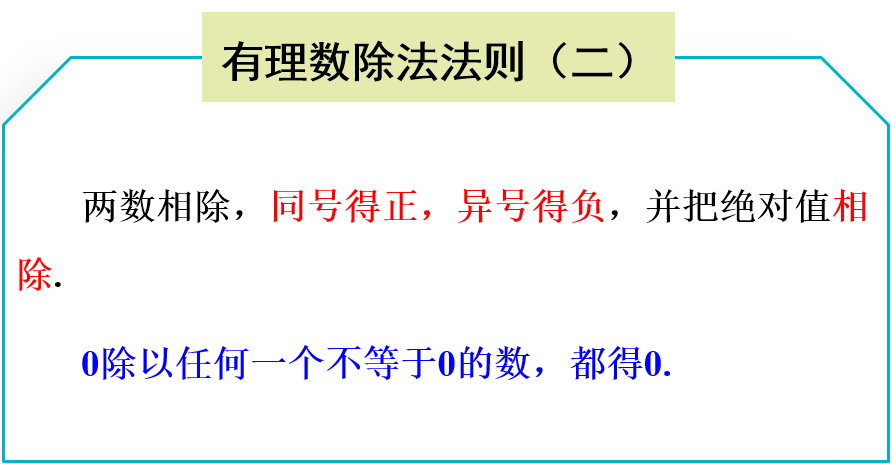
\includegraphics[width=.99\textwidth]{assets/division2.png}
        \end{figure}
    \end{columns}
\end{frame}

\begin{frame}{例题13}{知识点:除法}
    \begin{figure}
        \flushleft
        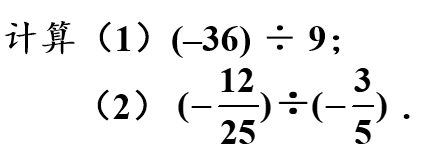
\includegraphics[width=.39\textwidth]{assets/div examp.png}
    \end{figure}
    \begin{figure}
        \flushleft
        \includegraphics<2>[width=.39\textwidth]{assets/div examp1.png}
    \end{figure}
\end{frame}

\begin{frame}{例题14}{知识点:除法乘法混合运算}
    \begin{block}{计算}
        \bmc{(-3)\times \dfrac{1}{3} \div(-\dfrac{1}{3})\times 3}\\

        \only<2>{\alert{9}}
    \end{block}
\end{frame}

\begin{frame}{例题15}{知识点:除法}
    \begin{figure}
        \flushleft
        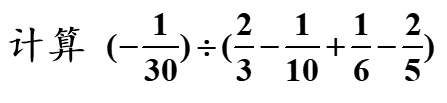
\includegraphics[width=.45\textwidth]{assets/examp14.png}
    \end{figure}
            \begin{figure}
                \includegraphics<2>[width=.99\textwidth]{assets/examp14-1.png}
            \end{figure}
            
            \begin{figure}
                \includegraphics<3>[width=.89\textwidth]{assets/examp14-2.png}
            \end{figure}
\end{frame}

\againframe{Question}

\subsection{有理数的乘方}
\begin{frame}
    \frametitle{有理数的乘方}

        \begin{itemize}
        \item<1-> Eggs
        \item<2-> Plants
        \note[item]<2>{Tell joke about plants.}
        \note[item]<2>{Make it short.}
        \item<3-> Animals
        \end{itemize}

        
        
        
\end{frame}

\subsection{有理数的混合运算}
\begin{frame}
    \frametitle{有理数的混合运算}
\end{frame}
\end{document}